\addtocontents{toc}{\vspace{\baselineskip}\noindent{\titlefont\bfseries\large III\quad Contributions}\par\vspace{0.3em}}
\chapter{MicroRTS Tournament Framework}
\label{chap:evaluation-framework}

Competition leaderboards change yearly with new opponent pools and maps, making direct comparison across editions unreliable. Moreover, as discussed in Section~\ref{subsec:competition}, the $2026$ competition shifted to LLM-based agents, precluding participation with this thesis's RL approach. This chapter introduces a reproducible tournament framework, inspired by the MicroRTS competition and anchored on its $2023$ edition. It comprises a tournament runner, twelve evaluation maps, fifteen benchmark agents spanning seven competition editions ($2017$--$2024$), and five ranking metrics.

\section{Tournament Infrastructure}
\label{sec:tournament-infrastructure}

The tournament pipeline (Figure~\ref{fig:tournament-architecture}) consists of three phases (configuration, execution, analysis), orchestrated by a unified Python command-line interface (CLI).

\paragraph*{1. Configuration:} a JSON file specifies all tournament parameters (maps, competing agents, games per matchup, time budgets, maximum game length, and optional flags for trace saving). This declarative format ensures full reproducibility of any tournament.

\paragraph*{2. Execution:} a Python tournament runner drives the MicroRTS Java simulation engine through a \emph{JPype} bridge (Chapter~\ref{chap:python_bridge}). The runner loads pre-compiled agent JARs at runtime. For each ordered pair of agents on each map, the engine plays a configurable number of games with alternating starting positions (avoiding positional bias) and records the outcome, game duration, and optional game traces; the concrete per-tournament game counts are reported with each experiment in Chapter~\ref{chap:results}. Games of the same matchup are vectorized using MicroRTS parallel environments to improve throughput, and matchup groups are distributed across SLURM (Simple Linux Utility for Resource Management) cluster jobs to balance computation time.

\paragraph*{3. Analysis:} a post-processing pipeline parses the raw CSV output into structured JSON, computes all five ranking metrics (Section~\ref{sec:metrics-used}) per map and globally, and generates PDF visualizations.

\begin{figure}[!ht]
    \centering
    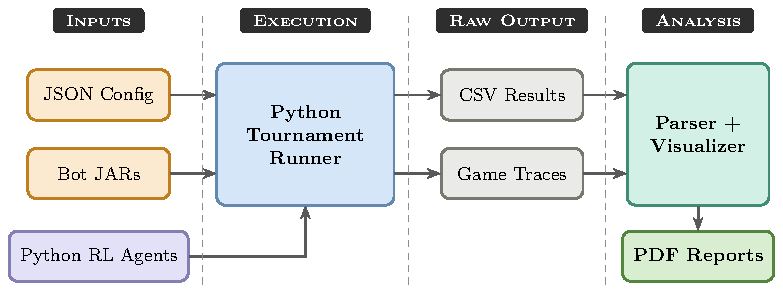
\includegraphics[width=\linewidth]{chapters/06_evaluation_framework/figures/tournament_architecture.pdf}
    \caption[Three-phase architecture of the tournament pipeline]{Three-phase architecture of the tournament pipeline.}
    \label{fig:tournament-architecture}
\end{figure}

\section{Evaluation Maps}
\label{sec:evaluation-maps}

The benchmark adopts the twelve maps (Table~\ref{tab:evaluation-maps}) of the IEEE CoG $2023$ MicroRTS competition\footnote{R. Oliveira, MicroRTS $2023$ competition, GitHub: \url{https://github.com/rubensolv/MicroRTS2023Competition}.}, split into two pools. The \emph{open pool} contains the eight publicly available maps that have remained the standard set across all competition editions, enabling direct comparison with published results. The \emph{closed pool} contains the four maps held out for the $2023$ edition, unknown to competitors before the event itself. These maps are excluded from training here, replicating the closed-pool conditions of the actual competition and providing a held-out generalization test.

The $2023$ edition is chosen as the anchor because it is the year RAISocketAI competed, making it the most relevant baseline for this thesis. The twelve maps span grid sizes from $8{\times}8$ to $64{\times}64$ and vary in starting conditions (number of bases, workers, and barracks), in terrain complexity (open arenas, choke points, dense maze layouts), and in resource distribution (symmetric, contested, or asymmetric). The \emph{Cycles} column reports the maximum game length, expressed in MicroRTS timesteps, which scales with grid size. Visual representations of all maps are provided in Appendix~\ref{app:maps}.

\begin{table}[!ht]
\centering
\caption[Characteristics of the twelve evaluation maps]{Characteristics of the twelve evaluation maps, ordered by grid size within each pool.}
\label{tab:evaluation-maps}
\renewcommand{\arraystretch}{1.2}
\setlength{\tabcolsep}{4pt}
\footnotesize
\begin{tabularx}{\textwidth}{@{} l c r c c c r >{\raggedright\arraybackslash}X @{}}
\toprule
\textbf{Map} & \textbf{Size} & \textbf{Cycles} & \textbf{B} & \textbf{W} & \textbf{Bar.} & \textbf{Res.\,/\,Total} & \textbf{Key Challenge} \\
\midrule
\multicolumn{8}{@{}l}{\textit{Open maps (available for training and evaluation)}} \\
\midrule
\emph{basesWorkers8x8A}        & $8{\times}8$   & $3\,000$ & $1$ & $1$ & $0$ & $5\,/\,40$   & Minimal; fast games; pure tactical micro \\
\emph{FourBasesWorkers8x8}     & $8{\times}8$   & $3\,000$ & $4$ & $4$ & $0$ & $20\,/\,280$ & Multi-base management; resource-rich \\
\emph{NoWhereToRun9x8}         & $9{\times}8$   & $4\,000$ & $1$ & $0$ & $0$ & $5\,/\,80$   & No workers; contested central resource line \\
\emph{basesWorkers16x16A}      & $16{\times}16$ & $4\,000$ & $1$ & $1$ & $0$ & $5\,/\,100$  & Similar to $8{\times}8$ variant with longer horizons \\
\emph{TwoBasesBarracks16x16}   & $16{\times}16$ & $4\,000$ & $2$ & $0$ & $2$ & $10\,/\,120$ & Pre-built barracks; early military production \\
\emph{DoubleGame24x24}         & $24{\times}24$ & $5\,000$ & $2$ & $4$ & $0$ & $10\,/\,284$ & Wall corridors; choke points; two-front war \\
\emph{BWDistantResources32x32}\textsuperscript{$\dagger$} & $32{\times}32$ & $6\,000$ & $1$ & $1$ & $0$ & $20\,/\,230$ & Large map; distant resources \\
\emph{BloodBath.scmB}\textsuperscript{$\dagger$}          & $64{\times}64$ & $8\,000$ & $1$ & $0$ & $0$ & $5\,/\,160$ & BroodWar conversion; complex maze terrain \\
\midrule
\multicolumn{8}{@{}l}{\textit{Closed maps (evaluation only)}} \\
\midrule
\emph{itsNotSafe}              & $15{\times}14$ & $4\,000$ & $1$ & $1$ & $1$ & $5\,/\,120$ & Central wall choke point; pre-built barracks \\
\emph{basesWorkers24x24A}      & $24{\times}24$ & $5\,000$ & $1$ & $1$ & $0$ & $5\,/\,100$ & Similar to $16{\times}16$ variant with longer horizons \\
\emph{basesWorkers32x32A}      & $32{\times}32$ & $6\,000$ & $1$ & $1$ & $0$ & $5\,/\,100$ & Similar to $24{\times}24$ variant with longer horizons \\
\emph{chambers32x32}           & $32{\times}32$ & $6\,000$ & $1$ & $1$ & $0$ & $5\,/\,260$ & Dense maze terrain; multiple chambers \\
\bottomrule
\multicolumn{8}{@{}l}{\scriptsize B = bases; W = workers; Bar. = barracks; Res.\,/\,Total = starting resources per player\,/\,total map resources.} \\
\multicolumn{8}{@{}l}{\scriptsize \textsuperscript{$\dagger$}Asymmetric resource distribution.} \\
\end{tabularx}
\end{table}

\section{Benchmark Agents}
\label{sec:benchmark-agents}

The benchmark spans seven competition editions ($2017$--$2024$)\footnote{The $2025$ edition was excluded because the competing agents' source code references were not yet publicly available in an accessible format at the time of writing.}. For each year, the highest-ranked open-source agent was selected (Table~\ref{tab:competition-agents-summary}), prioritizing paradigm diversity (rule-based, search-based, hierarchical, and DRL). Additional agents were included to cover distinct algorithmic families. All competition agents have been introduced in detail in Chapters~\ref{chap:historical-approach} and~\ref{chap:sota}.

These competition agents are complemented by four built-in MicroRTS agents (Table~\ref{tab:baseline-agents-summary}). Three of the four use fixed scripted strategies and establish a controlled difficulty floor against which all other methods can be compared. Tables~\ref{tab:baseline-agents-summary} and~\ref{tab:competition-agents-summary} list all selected agents with their key characteristics.

\renewcommand{\arraystretch}{1.15}
\setlength{\tabcolsep}{4pt}

\begin{table}[!htp]
\centering
\caption[Built-in MicroRTS baseline agents]{Built-in MicroRTS baseline agents used for controlled evaluation.}
\label{tab:baseline-agents-summary}
\small
\renewcommand{\arraystretch}{1.1}
\begin{tabularx}{\textwidth}{
  >{\raggedright\arraybackslash}p{1.5cm}
  >{\raggedright\arraybackslash}p{2.6cm}
  >{\raggedright\arraybackslash}X
  >{\raggedright\arraybackslash}p{4.2cm}
}
\toprule
\textbf{Paradigm} & \textbf{Agent} & \textbf{Strategy} & \textbf{Role in Evaluation} \\
\midrule
Rule & \urlref{https://github.com/Farama-Foundation/MicroRTS/blob/master/src/ai/RandomBiasedAI.java}{\textbf{RandomBiasedAI}} & Random actions with attack bias & Lower bound; difficulty floor \\
Rule & \urlref{https://github.com/Farama-Foundation/MicroRTS/blob/master/src/ai/abstraction/WorkerRush.java}{\textbf{WorkerRush}} & All-in worker rush & Early aggression test \\
Rule & \urlref{https://github.com/Farama-Foundation/MicroRTS/blob/master/src/ai/abstraction/LightRush.java}{\textbf{LightRush}} & All-in light rush (Listing~\ref{lst:rush-bot}) & Standard rush strategy test \\
Search & \urlref{https://github.com/Farama-Foundation/MicroRTS/blob/master/src/ai/mcts/naivemcts/NaiveMCTS.java}{\textbf{NaiveMCTS}} & MCTS $+$ CMAB & Search-based planning \\
\bottomrule
\end{tabularx}
\end{table}

\begin{table}[!htp]
\centering
\caption[Competition agents and GridNet baseline ($2017$--$2024$)]{Competition agents and GridNet baseline, selected for evaluation, spanning $2017$--$2024$.}
\label{tab:competition-agents-summary}

\begin{tabularx}{\textwidth}{
c
c
c
>{\raggedright\arraybackslash}p{2.8cm}
@{}>{\raggedright\arraybackslash}X
}
\toprule
\textbf{Year} & \textbf{Paradigm} & \textbf{Rank}\textsuperscript{$\dagger$} & \textbf{Agent} & \textbf{Key Characteristics} \\
\midrule

2017 & Hierarchical & 1st &
\urlref{https://github.com/nbarriga/microRTSbot}{\textbf{StrategyTactics}} &
Puppet Search with scripted action abstractions and NaiveMCTS for micro-management \\

2018 & Hierarchical & 1st &
\urlref{https://github.com/jr9Hernandez/TiamatBot}{\textbf{Tiamat}} &
Evolved action abstractions with real-time Strategy Selection Search (SSS)\footnotemark \\

2019 & Hierarchical & 1st &
\urlref{https://github.com/narsue/UTS_Imass}{\textbf{UtsImass}} &
Pre-game self-learning to optimize build parameters; in-game rule-based control with JPS pathfinding \\

2019 & Hierarchical & 2nd &
\urlref{https://github.com/AmoyZhp/MixedBotmRTS}{\textbf{MixedBot}} &
Integrates Tiamat for strategic search and CMAB-based tactical execution with dynamic time allocation \\

2019 & Search & 3rd &
\urlref{https://github.com/zuozhiyang/Droplet}{\textbf{Droplet}} &
Guided Naive Sampling: script-biased MCTS that steers search toward promising action sequences \\

2020 & Rule & 1st &
\urlref{https://github.com/Coac/coac-ai-microrts}{\textbf{CoacAI}} &
Heuristic economy management, defensive positioning, A* pathfinding \\

2021 & Rule & 1st &
\urlref{https://github.com/barvazkrav/mayariBot}{\textbf{Mayari}} &
Greedy per-action heuristic scoring with local distance estimation \\

2021 & DRL & N/A &
\urlref{https://github.com/Farama-Foundation/MicroRTS-Py}{\textbf{GridNet}} &
PPO with GridNet encoder-decoder; baseline for all DRL work in MicroRTS \\

2023 & Rule & 3rd &
\urlref{https://github.com/Jannis42/MicroRTSObiBotKenobi}{\textbf{ObiBotKenobi}} &
Role assignment and Dijkstra-based pathfinding with collision avoidance \\

2023 & DRL & 1st &
\urlref{https://github.com/sgoodfriend/rl-algo-impls}{\textbf{RAISocketAI}} &
PPO with the DoubleCone convolutional encoder-decoder architecture, self-play training, map-specific fine-tuning \\

2024 & Rule & 1st &
\urlref{https://github.com/MazzaAlessandro/TMA}{\textbf{TMA}} &
Four strategy combinations (attack/defense $\times$ worker/military), recalibrated every $500$ cycles \\

\bottomrule
\multicolumn{5}{@{}p{\textwidth}}{\scriptsize \textsuperscript{$\dagger$}Rank refers to the agent's placement in its listed competition year. GridNet did not enter any competition but serves as a DRL baseline.} \\
\end{tabularx}
\end{table}
\footnotetext{SSS searches over a small set of high-level strategies rather than individual unit actions.}

\section{Ranking Metrics}
\label{sec:metrics-used}

\subsection{Primary Metric: Win Rate}

The pairwise win rate between agents $i$ and $j$ is:
\begin{equation}
\mathrm{WR}(i, j) = \frac{w_{ij} + 0.5\, d_{ij}}{n_{ij}},
\end{equation}
where $w_{ij}$, $d_{ij}$, and $n_{ij}$ are respectively the wins, draws, and total games of agent $i$ against agent $j$. Draws contribute half a win to each player (standard round-robin convention).

The overall win rate of agent $i$ is the average across all opponents:
\begin{equation}
    \mathrm{WR}_i = \frac{1}{n-1} \sum_{j \neq i} \mathrm{WR}(i, j).
\end{equation}

\subsection{Complementary Game-Theoretic Metrics}
\label{subsec:game-theoretic}

Non-transitive cycles (A beats B, B beats C, C beats A) allow weak agents to artificially inflate win-rate scores. Win rate is therefore complemented with four game-theoretic metrics, computed both globally and per map. Each captures a different aspect of agent strength, as summarized in Table~\ref{tab:metrics-summary}. Appendix~\ref{app:game-theory} provides the mathematical formulations and a worked $4$-agent example illustrating how the four metrics produce complementary rankings of the same pool.

\begin{table}[!ht]
\centering
\caption[Ranking metrics and the evaluation question each addresses]{Ranking metrics and the evaluation question each addresses.}
\label{tab:metrics-summary}
\renewcommand{\arraystretch}{1.25}
\footnotesize
\begin{tabularx}{\textwidth}{@{}l l X@{}}
\toprule
\textbf{Metric} & \textbf{Perspective} & \textbf{Question} \\
\midrule
Win Rate & Aggregate performance & How often does the agent win overall? \\
Nash Averaging & Worst-case robustness & How well does the agent perform against an optimally adversarial opponent mix? \\
$\alpha$-Rank & Evolutionary stability & Can the agent's strategy resist invasion and dominate a competing population? \\
Copeland Score & Pairwise dominance & How many opponents does the agent beat head-to-head? \\
Regret & Robustness gap & How much worse does the agent perform than the pool's best counter against each opponent? \\
\bottomrule
\end{tabularx}
\end{table}

\vspace{-0.5em}

\paragraph*{Nash Averaging}~\cite{balduzziReevaluatingEvaluation2018} solves the win-rate matrix as a symmetric zero-sum meta-game and evaluates each agent by its expected payoff against the Nash equilibrium mixture. The resulting ranking is invariant to adding redundant or dominated agents. When multiple Nash equilibria exist, scores outside the equilibrium support are not unique. Agents that only beat weak opponents rank low; agents that hold up against the strongest competition rank high.

\paragraph*{$\alpha$-Rank}~\cite{omidshafieiARankMultiAgentEvaluation2019} models evolutionary dynamics over a population of agents. Starting from a monomorphic population playing a single strategy, it measures how easily a mutant using a different strategy can invade and take over. Agents that resist invasion and successfully displace others receive higher scores. Unlike Nash averaging, $\alpha$-Rank always produces a unique ranking.

\paragraph*{Copeland Score}~\cite{saariCopelandMethodRelationships1996} counts net pairwise victories: each head-to-head win contributes $+1$, each loss $-1$, and tied matchups $0$ to both agents, regardless of the margin. An agent that beats every opponent is a \emph{Condorcet winner}. Because only the direction of each matchup matters, not whether an agent wins 51\% or 99\%, the Copeland score captures dominance breadth independently of magnitude.

\paragraph*{Regret}~\cite{savageTheoryStatisticalDecision1951} measures how far an agent falls short of the best available alternative for each matchup. If another agent in the pool achieves 90\% win rate against opponent $j$ while a given agent only achieves 60\%, its regret for that matchup is 30\%. Both \emph{average regret} (overall consistency) and \emph{worst-case regret} (single most exploitable matchup) are reported.